\documentclass[a4paper,14pt]{extarticle}

% Путь до папки с общими шаблонами
\newcommand{\pathToCommonFolder}{/home/denilai/Desktop/LaTeX/Common}
% Название работы в титуле
\newcommand{\workname}{Отчет по практической работе №2}
% Название дисциплины в титуле
\newcommand{\discipline}{Анализ и концептуальное моделирование систем}
% Название кафедры в титуле
\newcommand{\kafedra}{Кафедра Практической и Прикладной Информатики}
% Тема работы в титуле
\newcommand{\theme}{Описание функций системы через диаграмму вариантов использования}
% Должность преподавателя в титуле
\newcommand{\rang}{доцент}
% ФИО преподавателя в титуле
\newcommand{\teacherfio}{В.~В.~Пяткин}


\usepackage{tabularx}



\usepackage{booktabs}
\newcolumntype{b}{X}
\newcolumntype{s}{>{\hsize=.5\hsize}X}
\newcommand{\heading}[1]{\multicolumn{1}{c}{#1}}

% Вставка заготовки преамбулы
% Этот шаблон документа разработан в 2014 году
% Данилом Фёдоровых (danil@fedorovykh.ru) 
% для использования в курсе 
% <<Документы и презентации в \LaTeX>>, записанном НИУ ВШЭ
% для Coursera.org: http://coursera.org/course/latex .
% Исходная версия шаблона --- 
% https://www.writelatex.com/coursera/latex/5.3

% В этом документе преамбула

% Для корректного использования русских символов в формулах
% пакеты hyperref и настройки, связанные с ним, стоит загуржать
% перед загрузкой пакета mathtext



% поддержка русских букв
% кодировка шрифта
%\usepackage[T2A]{fontenc} 
\usepackage{pscyr}

% использование ненумеровонного абзаца с добавлением его в содержаниеl

\newcommand{\anonsection}[1]{\section*{#1}\addcontentsline{toc}{section}{#1}}
\newcommand{\sectionunderl}[1]{\section*{\underline{#1}}}


% настройка окружения enumerate
\usepackage{enumitem}
\setlist{noitemsep}
\setlist[enumerate]{labelsep=*, leftmargin=1.5pc}

\usepackage{hyperref}

% сначала ставить \usepackage{extsizes} % Возможность сделать 14-й шрифт
% для корректной установки полей вставлять преамбулу следует в последнюю очередь (но перед дерективой замены \rmdefault)
\usepackage[top=20mm,bottom=25mm,left=35mm,right=20mm]{geometry} % Простой способ задавать поля

\hypersetup{				% Гиперссылки
	unicode=true,           % русские буквы в раздела PDF
	pdftitle={Заголовок},   % Заголовок
	pdfauthor={Автор},      % Автор
	pdfsubject={Тема},      % Тема
	pdfcreator={Создатель}, % Создатель
	pdfproducer={Производитель}, % Производитель
	pdfkeywords={keyword1} {key2} {key3}, % Ключевые слова
	colorlinks=true,       	% false: ссылки в рамках; true: цветные ссылки
	linkcolor=red,          % внутренние ссылки
	citecolor=black,        % на библиографию
	filecolor=magenta,      % на файлы
	urlcolor=blue           % на URL
}

%%% Работа с русским языком
\usepackage{cmap}					% поиск в PDF
\usepackage{mathtext} 				% русские буквы в формулах
\usepackage[T2A]{fontenc}			% кодировка
\usepackage[utf8]{inputenc}			% кодировка исходного текста
\usepackage[english,russian]{babel}	% локализация и переносы
\usepackage{indentfirst}
\frenchspacing

%для изменения названия списка иллюстраций
\usepackage{tocloft}


\renewcommand{\epsilon}{\ensuremath{\varepsilon}}
\renewcommand{\phi}{\ensuremath{\varphi}}
\renewcommand{\kappa}{\ensuremath{\varkappa}}
\renewcommand{\le}{\ensuremath{\leqslant}}
\renewcommand{\leq}{\ensuremath{\leqslant}}
\renewcommand{\ge}{\ensuremath{\geqslant}}
\renewcommand{\geq}{\ensuremath{\geqslant}}
\renewcommand{\emptyset}{\varnothing}

% Изменения параметров списка иллюстраций
\renewcommand{\cftfigfont}{Рисунок } % добавляем везде "Рисунок" перед номером
\addto\captionsrussian{\renewcommand\listfigurename{Список иллюстративного материала}}

\newcommand{\tm}{\texttrademark\ }
\newcommand{\reg}{\textregistered\ }


%%% Дополнительная работа с математикой
\usepackage{amsmath,amsfonts,amssymb,amsthm,mathtools} % AMS
\usepackage{icomma} % "Умная" запятая: $0,2$ --- число, $0, 2$ --- перечисление

%% Номера формул
%\mathtoolsset{showonlyrefs=true} % Показывать номера только у тех формул, на которые есть \eqref{} в тексте.
%\usepackage{leqno} % Нумереация формул слева

%% Свои команды
\DeclareMathOperator{\sgn}{\mathop{sgn}}

%% Перенос знаков в формулах (по Львовскому)
\newcommand*{\hm}[1]{#1\nobreak\discretionary{}
{\hbox{$\mathsurround=0pt #1$}}{}}


% отступ для первого абзаца главы или параграфа
%\usepackage{indentfirst}

%%% Работа с картинками
\usepackage{graphicx}  % Для вставки рисунков
\graphicspath{{images/}{screnshots/}}  % папки с картинками
\DeclareGraphicsExtensions{.pdf,.png,.jpg}
\setlength\fboxsep{3pt} % Отступ рамки \fbox{} от рисунка
\setlength\fboxrule{1pt} % Толщина линий рамки \fbox{}
\usepackage{wrapfig} % Обтекание рисунков текстом

%%% Работа с таблицами
\usepackage{array,tabularx,tabulary,booktabs} % Дополнительная работа с таблицами
\usepackage{longtable}  % Длинные таблицы
\usepackage{multirow} % Слияние строк в таблице

%%% Теоремы
\theoremstyle{plain} % Это стиль по умолчанию, его можно не переопределять.
\newtheorem{theorem}{Теорема}[section]
\newtheorem{proposition}[theorem]{Утверждение}

\theoremstyle{plain} % Это стиль по умолчанию, его можно не переопределять.
\newtheorem{work}{Практическая работа}[part]


 
 
\theoremstyle{definition} % "Определение"
\newtheorem{corollary}{Следствие}[theorem]
\newtheorem{problem}{Задача}[section]
 
\theoremstyle{remark} % "Примечание"
\newtheorem*{nonum}{Решение}



%%% Программирование
\usepackage{etoolbox} % логические операторы

%%% Страница

%	\usepackage{fancyhdr} % Колонтитулы
% 	\pagestyle{fancy}
%   \renewcommand{\headrulewidth}{0pt}  % Толщина линейки, отчеркивающей верхний колонтитул
% 	\lfoot{Нижний левый}
% 	\rfoot{Нижний правый}
% 	\rhead{Верхний правый}
% 	\chead{Верхний в центре}
% 	\lhead{Верхний левый}
%	\cfoot{Нижний в центре} % По умолчанию здесь номер страницы

\usepackage{setspace} % Интерлиньяж
\onehalfspacing % Интерлиньяж 1.5
%\doublespacing % Интерлиньяж 2
%\singlespacing % Интерлиньяж 1

\usepackage{lastpage} % Узнать, сколько всего страниц в документе.

\usepackage{soul} % Модификаторы начертания


\usepackage[usenames,dvipsnames,svgnames,table,rgb]{xcolor}


\usepackage{csquotes} % Еще инструменты для ссылок

%\usepackage[style=authoryear,maxcitenames=2,backend=biber,sorting=nty]{biblatex}

\usepackage{multicol} % Несколько колонок

\usepackage{tikz} % Работа с графикой
\usepackage{pgfplots}
\usepackage{pgfplotstable}

% модуль для вставки рыбы
\usepackage{blindtext}

\usepackage{listings}
\usepackage{color}


% для поворота отдельной страницы. Использовать окружение \landscape
\usepackage{pdflscape} 
\usepackage{rotating} 


\definecolor{mygreen}{rgb}{0,0.6,0}
\definecolor{mygray}{rgb}{0.5,0.5,0.5}
\definecolor{mymauve}{rgb}{0.58,0,0.82}


% пример импорта файла
%\lstinputlisting{/home/denilai/repomy/conf/distributions}

\lstset{
	language=Python,
	basicstyle=\footnotesize,        % the size of the fonts that are used for the code
	numbers=left,                    % where to put the line-numbers; possible values are (none, left, right)
	numbersep=5pt,                   % how far the line-numbers are from the code
	numberstyle=\tiny\color{mygray}, % the style that is used for the line-numbers
	stepnumber=2,                    % the step between two line-numbers. If it's 1, each line will be numbered
	% Tab - 2 пробела
	tabsize=2,    
	% Автоматический перенос строк
	breaklines=true,
	frame=single,
	breakatwhitespace=true,
	title=\lstname 
}



% установка размера шрифта для всего документа
%\fontsize{20pt}{18pt}\selectfont
\usepackage{extsizes} % Возможность сделать 14-й шрифт

\author{Кирилл Денисов}
\title{Практическая работа №2}
\date{\today}

% установка полуторного интервала
% \usepackage{setspace}  
% \onehalfspacing

% использовать Times New Roman
\renewcommand{\rmdefault}{ftm}


\begin{document}
	\thispagestyle{empty}
	
	% Вставка первого титульного листа
	%\newcounter{withouttheme}

%\setcounter{withouttheme}{<n>} установить значение счетчика  withouttheme для определения, нужна ли тема
%    {0} - нужна
%    {1} - не нужна

%\setcounter{withoutsubmissiondate}{<n>} установить значение счетчика  withoutsubmissiondate для определения, нужна ли дата представления к защите
%     {0} - нужна
%     {1} - не нужена
\begin{center}
	\begin{figure}[h!]
		\begin{center}
		%\vspace{-10ex}
		
\includegraphics[width=0.17\linewidth]{\pathToCommonFolder/gerb}
		%\caption{}\label{pic:first}
		%	\vspace{5ex}
		\end{center}	
	\end{figure}
 	\small	МИНОБРНАУКИ РОССИИ \\
	Федеральное государственное бюджетное образовательное учреждение\\
						высшего образования\\
\normalsize					
\textbf{«МИРЭА – Российский технологический университет»\\
						РТУ МИРЭА}\\
						\noindent\rule{1\linewidth}{1pt}\\
       Институт информационных технологий\\ %\vspace{2ex}
					\kafedra\\
		\vspace{3ex}
			\large \textbf{\workname}  \\
		%\vspace{1ex}
						по дисциплине\\ «\discipline» \\
		\vspace{3ex}
		\ifnum \value{withouttheme}=0 {
			\textbf{Тема работы:}\\ <<\theme>>
		}
		\else {}
		\fi
\vspace{10ex}
\small
\begin{table}[h!]
\begin{tabular}{lp{0.6\linewidth}l}
	\textbf{Выполнил:} & студент группы ИВБО-02-19 & \\ 
	& & \studentfio \\%Д.~Н.~Федосеев\\%А.~М.~Сосунов\\%К.~Ю.~Денисов\\%И.~А.~Кремнев
	\textbf{Принял:} & \rang & \\
	& & \teacherfio \hfill\\
\end{tabular}
\end{table}
\end{center}
\ifnum \value{withoutsubmissiondate}=0 {
	\begin{flushleft}
		Работа представлена к защите <<\rule{3ex}{1pt}>>\rule{10ex}{1pt} 202\rule{1ex}{1pt} г.\hfill
	\end{flushleft}
\else {}
\fi

\normalsize
\begin{center}	
\vfill
Москва 2022
\end{center}

	
	\newpage
	\tableofcontents
	\newpage
	
\section{Цели и задачи работы}
Цель работы: изучить основные элементы и правила построения диаграммы
вариантов использования.

Задачи: описать функции рассматриваемой системы с помощью диаграммы
вариантов использования.

Нотация: UML (Use case diagram).

Программное обеспечение: Draw.io.
\section{Индивидуальный вариант №6}
\begin{problem}
Построить диаграмму вариантов использования по следующему описанию: <<Клиент банка может пополнить счет, в случае отсутствия счета предварительно открыв его, или снять деньги со счета, с возможностью его закрытия>>. В каждом из описанных действий участвует операционист банка и кассир.
\nonum В соответствии с предложенным описанием, составим диаграмму вариантов использования в нотации Use Case языка UML. См. рисунок \ref{img:usecase} в \hyperref[tam]{Приложении А}.
Таблица, заполненная на основе диаграммы вариантов испльзования находится в \hyperref[tam]{Приложении А}.

\end {problem}
\begin{problem}
	Описать спецификацию функций рассматриваемой системы с учетом
	индивидуального варианта учебного проекта.
	Перед построением диаграммы необходимо задокументировать потоки
	событий в системе.
	Поток событий – процесс обработки данных, реализуемый в рамках одного
	или нескольких вариантов использования. Описание потока включает
	информацию о том, какие обязанности возлагаются на актеров, а какие на
	систему.
	\nonum
	Опишем спецификацию функций оптового предприятия, являющегося дистрибьюторской компанией и осуществляющей реализацию крупных партий товара, приобретенного у товаропроизводителя. Таблица спецификаций находится в \hyperref[tam]{Приложении А}.	
	

	Опишем потоки событий, которые имеют место при данном взаимодействии поставщика-товаропроизводителя, компании-дистрибьютора и клиентов (розничный посредник или предприятие, осуществляющее розничную торговлю).
	\begin{itemize}
		\item В случае, если и поставщика, и оптовую компанию удовлетворяют условия совместной работы, то они заключают договор о сотрудничестве. При этом на дистрибьютора возлагается обязанность следовать заранее избранной товаропроизводителем рыночной стратегии, при этом получая право действовать от имени товаропроизводителя.
		\item После заключения договора о сотрудничестве и проведением дистрибьютором маркетинговой компании и изучения рынка сбыта, товаропроизводитель передает право на реализацию собственного товарного продукта, при этом чаще всего оптовая компания не пользуются правом приобретения товара в полную собственность.
		\item Для составления конкуренции на рынке, компании-дистрибьютору необходимо проводить широкую маркетинговую и пропагандистскую компанию, расширять клиентскую базу и  использовать инструменты мерчандайзинга с целью популяризации товара и завоевания рынков сбыта, создания и развития сети распространения товарной продукции.
		\item Если частный клиент в лице розничного предприятия или дилера заинтересовался услугами компании-дистрибьютора, то он так же может заключить договор о сотрудничестве. Клиент руководствуется возможностью получения максимальной выгоды и построения надежных деловых отношений при выборе дистрибьюторской компании.
		\item Компания-дистрибьютор возлагает на себя обязанность по своевременной и бесперебойной поставке товарного продукта в заранее определенных размерах, решении логистических вопросов.		
	\end{itemize}
	Составим диаграмму вариантов использования согласно спецификации функций и в соответствии с потоками событий. Диаграмма расположена в \hyperref[tam]{Приложении А}, рисунок \ref{img:usecase2}.

\end {problem}
\section{Вывод}
В ходе данной практической работы был изучена спецификация функций изучаемой системы, рассмотрены принципы и правила построения диаграммы вариантов использования в нотации UML (Use Case). Полученные знания применены на практике.

\newpage
{\centering
\vspace{-10ex}
\small
\anonsection{ПРИЛОЖЕНИЕ А}}

\label{tam}

	\begin{longtable}{|m{0.25\linewidth}|m{0.24\linewidth}|m{0.44\linewidth}|}
	\caption{{Описание взаимодействий актеров и вариантов использования}} \label{tab:long} \\
	
	\hline \multicolumn{1}{|c|}{\textbf{Актер/ВИ}} & \multicolumn{1}{c|}{\textbf{Тип связи}} & \multicolumn{1}{c|}{\textbf{Вариант использования}} \\ \hline 
	\endfirsthead
	
	\multicolumn{3}{c}%
	{{\bfseries \tablename\ \thetable{} -- продолжение}} \\
	\hline \multicolumn{1}{|c|}{\textbf{Актер/ВИ}} & \multicolumn{1}{c|}{\textbf{Тип связи}} & \multicolumn{1}{c|}{\textbf{Вариант использования}} \\ \hline 
	\endhead
	
	\hline \multicolumn{3}{r}{\textit{Продолжение на следующей странице}} \\
	\endfoot
	
	\hline \hline
	\endlastfoot
	\multirow{4}{\linewidth}{Клиент} & Направленная   ассоциация & Пополнение счета \\ \cline{2-3}
	& Направленная   ассоциация & Снятие средств со счета \\ \cline{2-3}
	& Направленная   ассоциация & Открытие счета физического лица \\ \cline{2-3}
	& Направленная   ассоциация & Закрытие счета физического лица \\ \cline{2-3}
	& Ненаправленная ассоциация & Передача денежных средств \\ \cline{2-3}
	& Ненаправленная ассоциация & Предоставление банковской карты \\ \cline{2-3}
	& Ненаправленная ассоциация & Предоставление реквизитов счета \\ \cline{2-3}
	& Ненаправленная ассоциация & Предоставление оригиналов и копий документов \\ \cline{2-3}
	& Ненаправленная ассоциация & Предоставление свидетельства о присвоении ИНН \\ \cline{2-3}
	& Ненаправленная ассоциация & Предоставление заявления об открытии счета \\ \hline
	Кассир       & Ненаправленная ассоциация & Внесение изменений в БД \\ \hline
	Операционист & Ненаправленная ассоциация & Внесение изменений в БД \\ \hline
	\multirow{2}{\linewidth}{Внесение изменений в БД} & Обобщение & Пополнение счета \\ \cline{2-3}
	& Обобщение & Снятие средств со счета \\ \hline
	\multirow{2}{\linewidth}{Изменение статуса вклада} & Обобщение & Открытие вклада физического лица \\ \cline{2-3}
	& Обобщение & Закрытие вклада физического лица \\ \hline
	\multirow{3}{\linewidth}{Открытие счета физического лица} & Включение & Предоставление оригиналов и копий документов \\ \cline{2-3}
	& Включение & Предоставление свидетельства о присвоении ИНН \\ \cline{2-3}
	& Включение & Предоставление заявления об открытии счета \\ \hline
	\multirow{2}{\linewidth}{Пополнение счета} & Включение & Передача денежных средств \\ \cline{2-3}
	& Включение & Предоставление реквизитов счета \\ \hline
	
	\multirow{2}{\linewidth}{\small Предоставление банковской карты} & Расширение & Предоставление реквизитов счета \\ \cline{2-3}
	& Расширение & Передача денежных средств  \\ \hline
	Снятие средств со счета & Включение & Предоставление реквизитов счета \\ \hline \newpage
	\multirow{2}{\linewidth}{Закрытие счета} & Расширение & Снятие средств со счета \\ \cline{2-3}
	& Расширение & Открытие счета физического лица \\ \hline	
\end{longtable}

\begin{figure}[h]
	\centering
	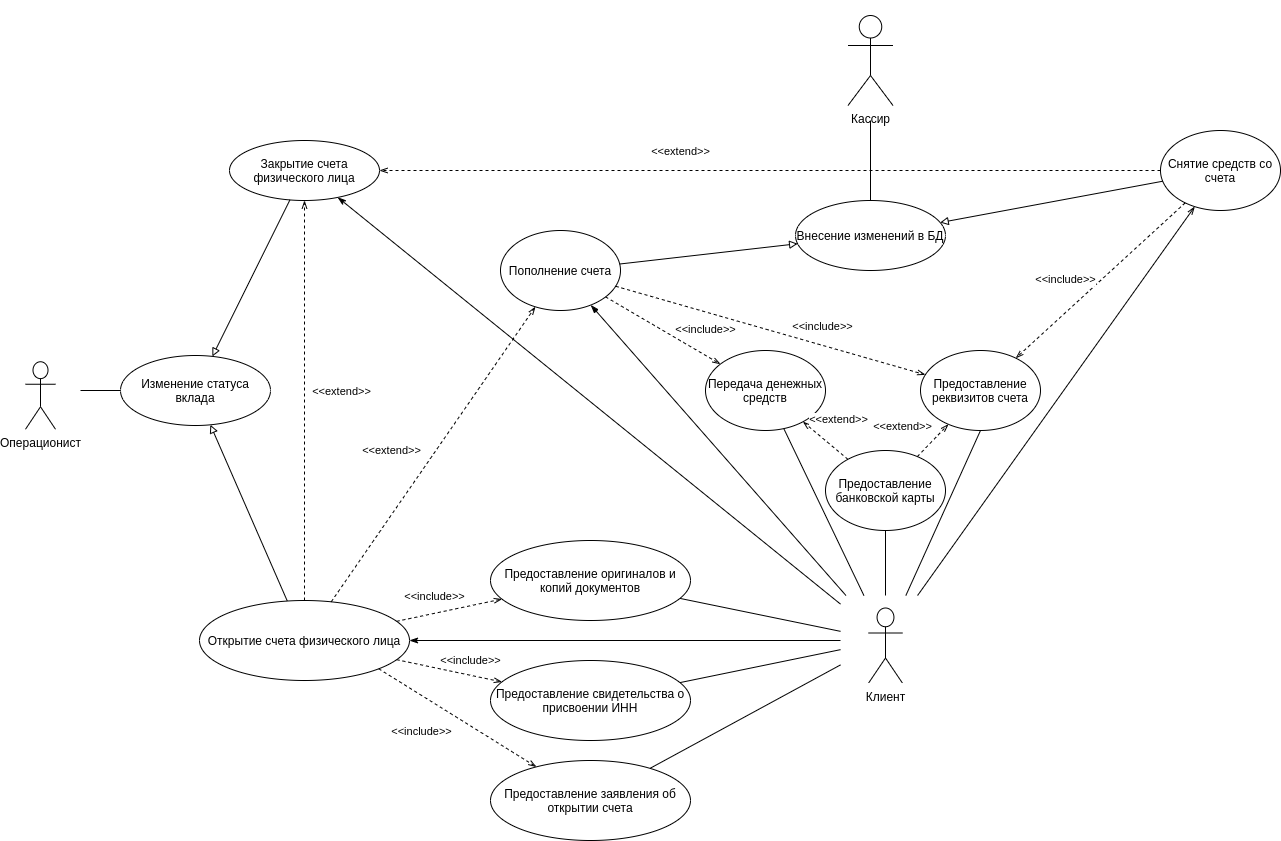
\includegraphics[width=1\linewidth]{usecase}
	\caption{Диаграмма вариантов использования к заданию 1}
	\label{img:usecase}
\end{figure}

\begin{table}
	\caption{Спецификация функций системы}
	\begin{tabular}{|c|m{0.6\linewidth}|}
		\hline
		\textbf{Субъект/Система} & \textbf{Функции} \\ \hline
		Клиент & Составление договора о сотрудничестве с дистрибьюторской компанией \\  \hline
		Клиент & Приобретение партий товара у дистрибьютора с целью продажи в розницу \\ \hline
		Товаропроизводитель & Заключение дистрибьюторского договора \\ \hline
		Товаропроизводитель & Организация оптовых поставок дистрибьютору \\ \hline
		Компания-дистрибьютор & Выработка бизнес-стратегии по увеличению товарооборота, привлечению новых клиентов \\ \hline
		Компания-дистрибьютор & Построение взаимодействия с клиентами с целью реализации товара \\ \hline
		Компания-дистрибьютор & Ведение рекламной политики \\ \hline			
	\end{tabular}
	
	\label{tab:func_spec}
\end{table}
\begin{figure}[tpb]
	\centering
	\vspace{2ex}
	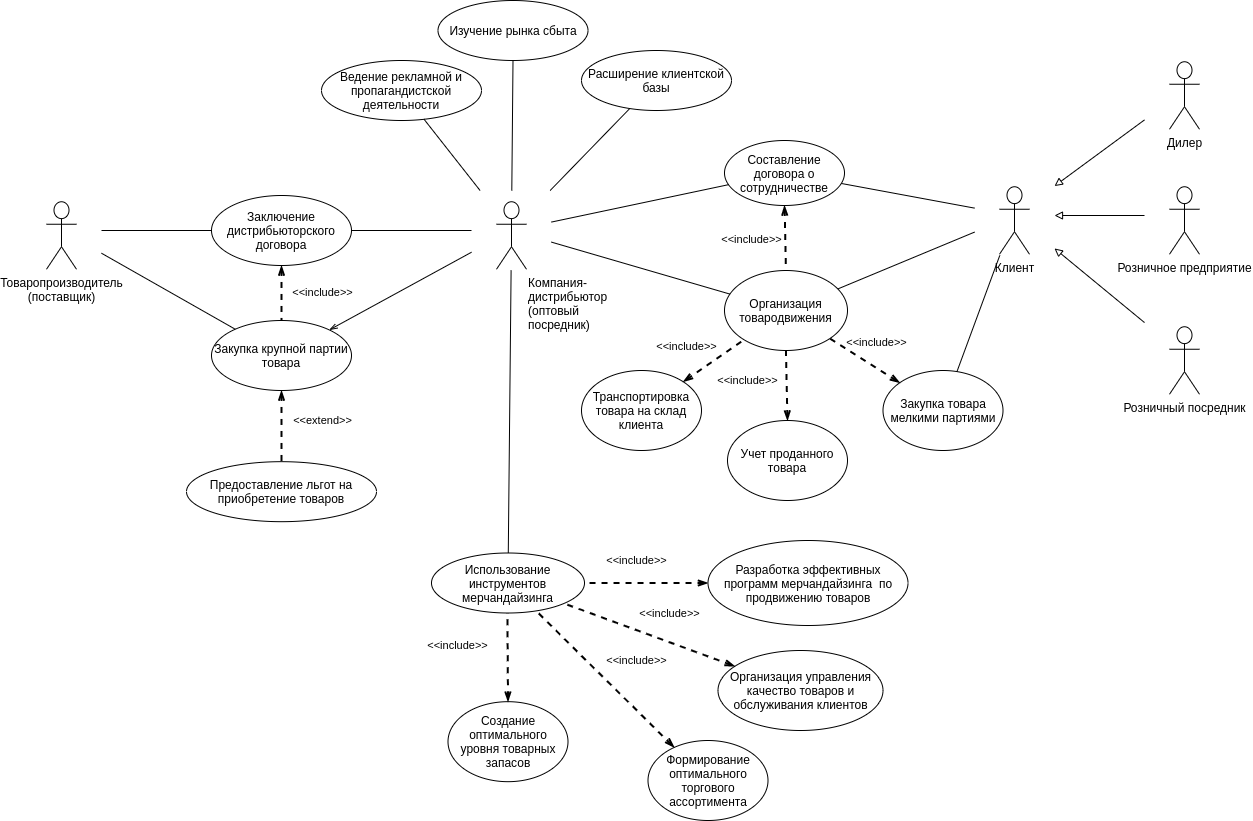
\includegraphics[width=0.8\linewidth]{usecase2}
	\caption{Диаграмма вариантов использования к заданию 2}
	\label{img:usecase2}
\end{figure}

\end{document}


